\begin{figure*}[ht!]
    \centering
    \includegraphics[width=\textwidth]{figures/solution/quantization_flow_img.pdf}
    \caption{
    \small 
        A high-level illustration of the quantization process in \sys.
    }
    \label{fig:quantizer}    
\end{figure*}



\section{\quantizer}
\label{sec:quantization}

This section outlines the design and implementation of the \quantizer. An overview of \quantizer's workflow is shown in \autoref{fig:quantizer}. First, the \quantizer ranks model parameters according to their magnitude and sensitivity (\S~\ref{sec:ranking}). Based on the ranking, the parameters are then partitioned into three groups (\S~\ref{sec:pruneandprotect}). The least important parameters are pruned, the most important ones are protected with high precision, while the remaining parameters are quantized using our novel non-uniform quantization approach (\S~\ref{sec:nonuniform}). 







\subsection{Metrics for Parameter Ranking}
\label{sec:ranking}
First, we need to rank parameters by importance in order to assign them for protection, pruning, or quantization.

The two popular metrics used to determine the importance of parameters are magnitude and sensitivity. Magnitude-based ranking approaches simply use the parameter magnitude as an importance score~\cite{han2015learning}. The magnitude score $I_m(w)$ for parameter $w$ is defined as $I_m(w) = |w|$. Sensitivity-based ranking approaches attempt to estimate the impact on the end-to-end loss value when a parameter is altered \cite{lecun1989optimal,dong2019hawq}. In this paper, we use the first-order Taylor series approximation formulation of sensitivity for the sake of computational efficiency. 
The sensitivity score is defined as $I_s(w) = |\nabla\mathcal{L}(w) w|$, where $\mathcal{L}$ represents the loss function and $\nabla\mathcal{L}(w)$ is the gradient of weight $w$ with respect to the loss function. It has been shown that magnitude-based parameter ranking approaches perform poorly in the early stage of training~\cite{when-to-prune}. On the other hand, as we approach convergence, gradients start to diminish, making the sensitivity metric less reliable. 




To address the above limitations, we propose to use a combination of sensitivity and magnitude to get a reliable ranking throughout the training process. \cref{fig:param-dist} shows the distribution of parameters across the two ranking dimensions for a ResNet152 model trained on Imagenet data. While there is a strong correlation between magnitude and sensitivity, we observe a significant number of outliers, which have a high magnitude score but a low sensitivity score or vice versa. By ranking parameters across both the metrics, \sys can identify and preserve these parameters.


\begin{figure}
    \centering
    \begin{subfigure}{1\linewidth}
    \begin{subfigure}{0.49\linewidth}
        \centering
        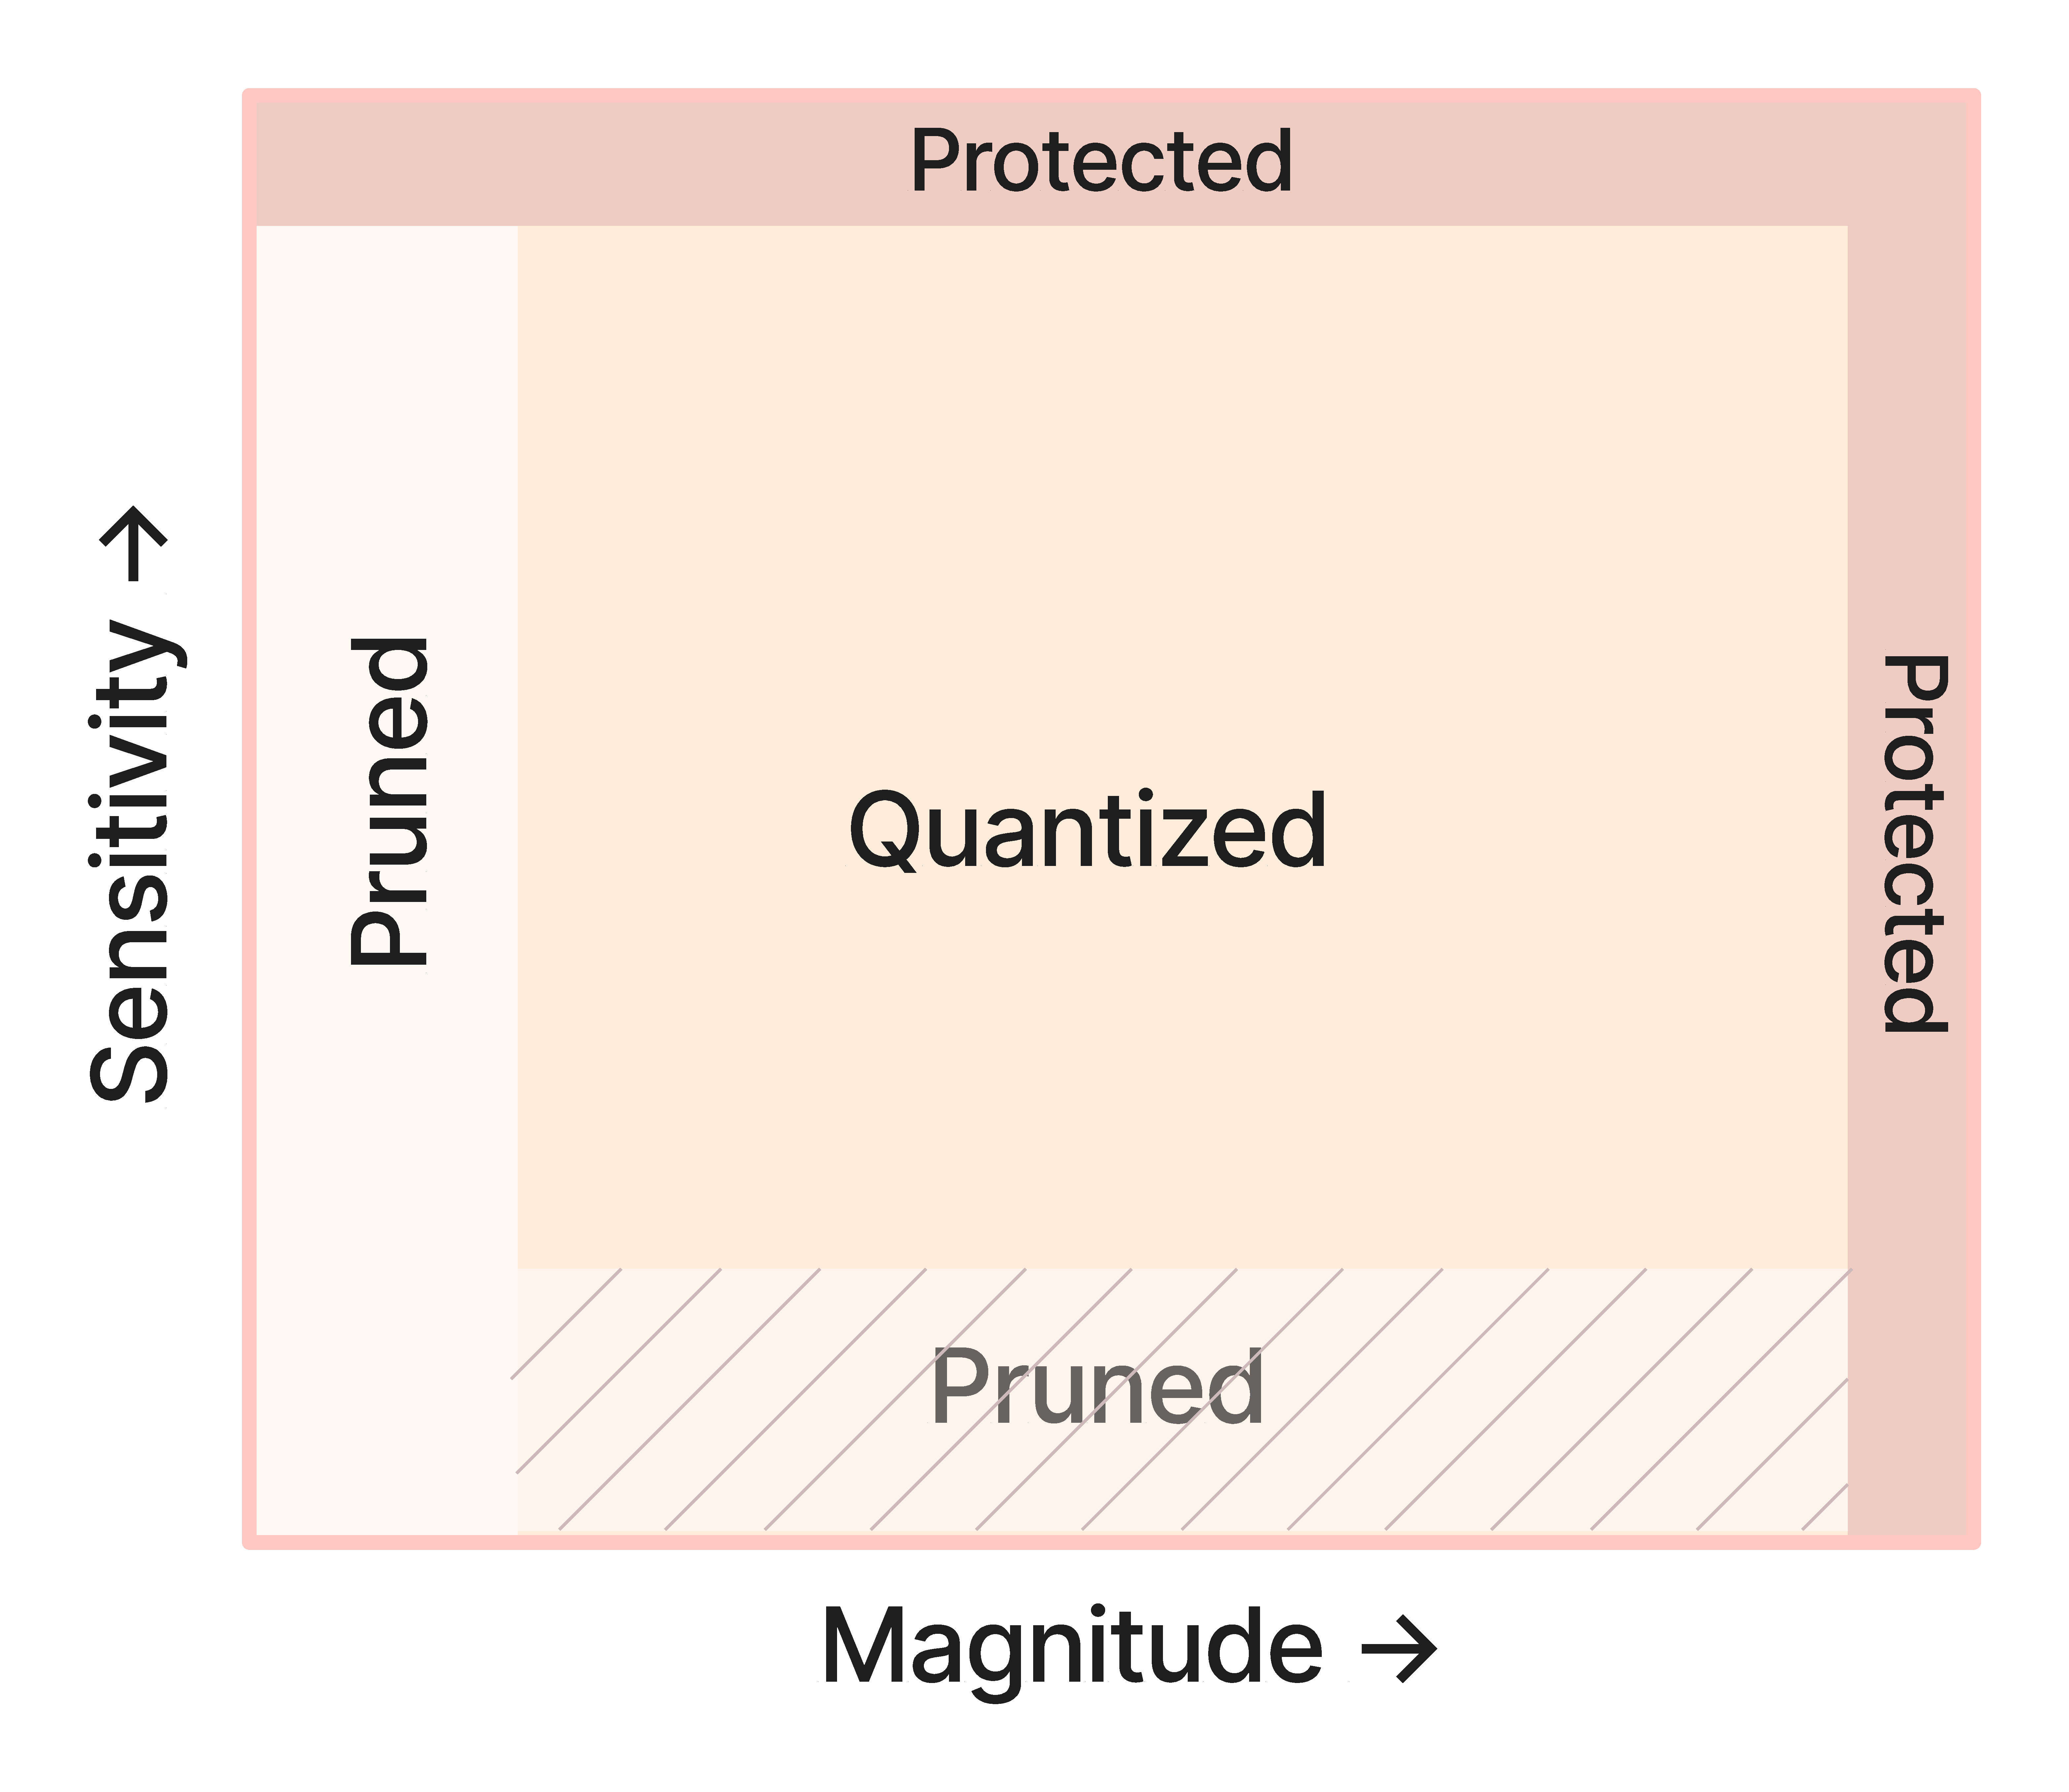
\includegraphics[width=0.95\linewidth]{figures/solution/parm_grid_img.pdf}
        \caption{\small Parameter partitioning schema in \sys.}
        \label{fig:param-grid}
    \end{subfigure}
    \hfill
    \begin{subfigure}{0.49\linewidth}
        \centering
        \includegraphics[width=0.9\linewidth]{figures/solution/scatter_plot.png}
        \caption{\small{Parameter distribution for ResNet152.}}
        \label{fig:param-dist}
    \end{subfigure}
    \end{subfigure}
    \caption{\small Model parameters are partitioned into three groups for pruning, protection, and quantization by jointly evaluating magnitude and sensitivity scores.}
    \vspace{-1em}
\end{figure}


For efficient sensitivity computation, we reuse gradients computed during the training process for sensitivity estimates and asynchronously copy the gradients to pinned CPU memory to avoid GPU memory overhead. We discuss implementation details in \cref{app:sensitivity-computation}. 




\subsection{Parameter Partitioning}
\label{sec:pruneandprotect}

Given the magnitude and sensitivity score for each model parameter, the \quantizer partitions the parameters into one of the three groups (\cref{fig:param-grid}). 

\noindent\textbf{Protection.}
\sys preserves the most important model parameters in the high precision \texttt{bfloat16} format.
Recent quantization studies~\cite{llm-int8, dash2020hessian} show a significant reduction in quantization error when a few important weights are protected. Our experiments suggest that protecting a small fraction (0.05-0.1\%) of both the highest magnitude and sensitivity parameters provides the best performance. The precise protection fraction is determined dynamically by the \qcm. Based on the fraction ($F_{\text{prot}}$) of parameters to be protected, we identify the minimum magnitude and sensitivity thresholds (quantiles) for a parameter to qualify for protection. 



\noindent\textbf{Pruning.} We prune the least significant model parameters, based on the pruning fraction $F_{\text{prun}}$ (typically between 10-40\%) and the pruning metric, magnitude or sensitivity. An important design consideration is the granularity level at which the pruning is performed. Layer-level pruning can degrade model quality due to different redundancy levels across the network layers.  Conversely, global pruning may disproportionately affect different layer types (e.g., Convolution, Attention, Linear) due to varied weight distributions. To tackle this, we perform {\em per-layer type} pruning, i.e. using the same pruning fraction across all layers of a given type. We observed that in GPT-2 Medium, we can eliminate up to 30\% parameters with a minimal effect on the model's quality.









\subsection{Efficient Parameter Partitioning via Quantile Sketches} 
\label{app:quantile}

Computing quantiles required for determining pruning and protection thresholds can be costly, especially for large models due to the log-linear time complexity of the operation. Moreover, in cases where models are trained via model parallelism, and parameters are distributed across different worker groups, computing global quantiles can be quite challenging. %


To facilitate efficient partitioning of model parameters, we use a sketch-based quantile estimation algorithm that is a simplified and parallelized version of DDSketch~\cite{ddsketch}. This enables us to compute approximate quantile estimates in linear time with a configurable $\alpha$-relative-error bound, that is, the sketch produces an estimated quantile value corresponding to the quantile value $x_q$ such that $|\tilde{x_q} - x_q| \leq \alpha x_q$. For computing protection and pruning thresholds, that require tail quantiles, DDSketch's relative error bounds outperform alternative quantile sketches that guarantee rank error. Furthermore, the quantile sketches are mergeable, which simplifies the computation of global quantile estimates from individual model shards.

The sketching algorithm transforms the input values into a logarithmic space and then divides them into an equal-width histogram (\cref{fig:log-sketch-transform}). Due to the use of a logarithmic scale, we achieve varying levels of detail for different ranges of the original values. Specifically, smaller original values will land in narrower bins, while larger values will fall into broader bins. This allows the sketch to provide the $\alpha$-relative error property of the sketch. To produce quantile estimates, the sketch sums up the buckets until it finds the bucket containing the desired quantile value.

Algorithm \ref{algo:quantile-sketch} describes the parallelizable version of DDSketch \cite{ddsketch} optimized for GPU execution. We forgo the bucket merging step in the original DDSketch for ease of parallelization. This has limited impact in practice, as we observe that the number of buckets does not exceed a few thousand even for models with hundreds of millions of parameters with a strict relative error bound of 1\%. We implement a highly parallelized version of this algorithm using Pytorch that can run on GPUs. We observe a 3-4$\times$ speed-up compared to off-the-shelf GPU-enabled implementation provided by CuPy \cite{cupy} while using significantly less memory.

\begin{figure}
    \centering
    \includegraphics[width=\linewidth]{figures/solution/log_sketch_transformation_img.pdf}
    \vspace{-1em}
    \caption{
        \small{
        {DDSketch's log space transformation creates a histogram with value-dependent bucket width.}
        }
    }
    \label{fig:log-sketch-transform}
\end{figure}

\begin{algorithm}
\caption{GetQuantileSketchHistogram}
\begin{algorithmic}[1]
\REQUIRE $X$ \COMMENT{Input list}
\REQUIRE $\alpha$ \COMMENT{Relative Error Bound}
\STATE $\gamma \leftarrow (1 + \alpha) / (1 - \alpha)$ \\
\STATE Define $X_q$ as an empty array \\
\FORALL{$x$ in $X$}
    \STATE Append $\lceil \log_{\gamma}(x) \rceil$ to $X_q$
\ENDFOR
\STATE $(\texttt{bucket\_vals}, \texttt{bucket\_counts}) \leftarrow \texttt{unique}(X_q)$
\RETURN $\texttt{bucket\_vals}, \texttt{bucket\_counts}$
\end{algorithmic}\label{algo:quantile-sketch}
\end{algorithm}



\subsection{Non-uniform Quantization via Approximate K-Means Clustering}
\label{sec:nonuniform}
The remaining model parameters that are not pruned or protected go through quantization. 
Quantization reduces the precision of model parameters to lower-bit representations (e.g., from 32-bit floating-point to 8-bit integers), leveraging redundancy and noise tolerance in large networks. Uniform quantization strategies create equally spaced quantization levels across the parameter space, while non-uniform quantization approaches use varying intervals between levels to adapt to the parameter distribution. 

Non-uniform quantization techniques, such as via \kmeans clustering~\cite{checknrun, gobo, deep-compression}, generally provide better compression and model quality. However, they have seen limited adoption in checkpoint compression systems due to their computational complexity. For instance, GOBO~\cite{gobo}, that utilizes a variant of \kmeans clustering, takes roughly 50 minutes to quantize a small model like ResNet-18 (11.7M parameters).



\begin{algorithm}
\caption{Approximate K-Means Clustering}
\begin{algorithmic}[1]
\REQUIRE $X$ \COMMENT{Input data points}, $k$ \COMMENT{Number of clusters}
\REQUIRE $\alpha$ \COMMENT{Relative error}, $\sigma$ \COMMENT{Linear combination factor}
\STATE $X_q$, $C_q$ $\leftarrow$ \texttt{GetQuantileSketchHistogram}($X$, $\alpha$) \COMMENT{Obtain log sketch histogram \cref{algo:quantile-sketch} for coarse grain clustering. $X_q$ are the histogram bucket centers and $C_q$ are the corresponding frequencies.}
\STATE  $\hat{X_q}$, $\hat{C_q}$ $\leftarrow$  \texttt{Normalize}($X_q$), \texttt{Normalize}($C_q$)
\STATE $W = \sigma * \hat{C_q} + (1 - \sigma) * |\hat{X_q}|$  \COMMENT{Compute sample weight for histogram buckets according to frequency and magnitude} 
\STATE $\texttt{centers}$ $\leftarrow$ \texttt{WeightedKMeans}($X_q$, $W$, $k$)  \COMMENT{Perform weighted k-means++ on histogram keys and values}  
\RETURN $\texttt{centers}$
\end{algorithmic}\label{algo:kmeans}
\end{algorithm}

\minihead{Approximate \kmeans Clustering}
We introduce a novel non-uniform quantization method leveraging approximate K-means clustering, which strikes a balance between quantization quality and computational efficiency. Our key insight is to perform K-means clustering on histogram buckets of the parameters, rather than on the raw parameters themselves. This significantly reduces the computational burden of K-means clustering, resulting in up to 65$\times$ speedup compared to the standard implementation in CuML (\S~\ref{sec:ablations}). 



\cref{algo:kmeans} describes the two-step quantization algorithm. First, we group model parameters into coarse-grain buckets, utilizing the same log-space projection approach in DDSketch. We then perform weighted k-means clustering, where the histogram bins serve as the data and their heights as sample weights, to establish quantization boundaries. Two key optimizations enhance this clustering performance:

\begin{figure}
    \centering
    
\includegraphics[width=\linewidth]{figures/solution/two_step_quantization_img.pdf}
        \vspace{-1em}
    \caption{
        \small{
        {Two-step quantization: 
        (1) group model parameters into coarse-grained buckets with sketch-based histogram computation. (2) cluster parameter buckets using sample weighted K-means clustering.}
        }}
    \label{fig:two-step-quantization}
\end{figure}

\begin{algorithm}
\caption{Weighted K-Means++ Initialization}
\begin{algorithmic}[1]
\REQUIRE $X$ \COMMENT{Input data points}
\REQUIRE $W$ \COMMENT{Input sample weights}
\REQUIRE $k$ \COMMENT{Number of clusters}
\STATE $C \leftarrow X[ \texttt{random\_choice}(W)]$ \COMMENT{Initialize the first centroid randomly according to weights}
\FOR{$i$ in $2$ to $k$}
    \STATE $D \leftarrow \texttt{min\_distance}(X, C)$ \COMMENT{Compute distance of each point to nearest centroid}
    \STATE $D \leftarrow D \cdot W$ \COMMENT{Weight the distances}
    \STATE $P \leftarrow D / \texttt{sum}(D)$ \COMMENT{Compute probabilities}
    \STATE $C \leftarrow C \cup X[ \texttt{random\_choice}(P)]$ \COMMENT{Select new centroid}
\ENDFOR
\RETURN $C$
\end{algorithmic}\label{algo:initialize}
\end{algorithm}


First, we introduce an additional parameter, $\sigma$, to our weighted \kmeans to help balance the allocation of resolution between high-importance parameters with low frequency and high-frequency parameters with low importance. Usually, non-uniform clustering offers increased resolution to denser parameter spaces. However, for neural network parameters, this would allocate greater resolution to values near zero. To address this, we calculate the sample weight of a bucket, $b^{i}$, as a linear combination of the bucket's normalized frequency and magnitude: $w^{i} = \sigma * b^{i}_{\text{freq}} + (1 - \sigma) * b^{i}_{\text{mag}}$ (see line 2 in \cref{algo:kmeans}). Our observations suggest that values of $\sigma$ in the range $0.1-0.4$ generally provide the best compression results. We use $\sigma=0.2$ for all experiments.


Second, the success of the \kmeans clustering algorithm relies heavily on proper initialization. Inappropriate initialization can lead to suboptimal solutions and slower convergence. K-means++~\cite{kmeanspp} addresses this by ensuring the initial centroids are uniformly distributed across the space, often leading to near-optimal solutions with a single round of clustering. We extend the K-means++ \cite{kmeanspp} algorithm for initialization with support for sample weights, \Cref{algo:initialize} provides a sketch of this process. 










\minihead{Error Analysis} In the first step of the quantization algorithm, we create a histogram using DDSketch's log-space projection approach, which provides a configurable $\alpha$-relative error bound. Using this approach, we formally show that the difference between optimal loss of \kmeans clustering over raw inputs $X$ and its histogram counterpart $\tX$ is bounded by $\alpha$. We can further show that when the clustering is performed with sample-weighted k-means++, then the expected loss over $\tX$ is bounded by the optimal loss over $X$ and an additional term related to $\alpha^2$ (\cref{app:kmeans}).















\subsection{Efficient Sensitivity Computation} 
\label{app:sensitivity-computation}
To save computational resources, we reuse gradients computed during the training process for sensitivity estimates instead of calculating them separately. To avoid any GPU memory overhead, we asynchronously copy the gradients to pinned CPU memory as soon as the backward pass is completed. The gradient copy operation is overlapped with the optimizer step, data loading, and forward pass of the next batch, making the overhead of this operation negligible as shown in \cref{fig:gradient-copy-timeline}. The copied gradient values are accumulated on the CPU using an exponential moving average $\text{EMA}^{t}_{g_w} = \beta * g^{t}_w + (1 - \beta) * \text{EMA}^{t - 1}_{g_w}$, where $\text{EMA}^{t}_{g_w}$ is the exponential moving average of the gradient $g_w$ at timestep $t$. We set the value of $\beta$ to be $0.9$ in all our experiments to emphasize the recent gradients. The gradient copy mechanism is only invoked for a limited preconfigured number of batches before checkpointing is scheduled to be performed to further avoid any impact on steady-state throughput. We identify that typically recording gradients for fifty batches is sufficient to get good sensitivity estimates. 

\begin{figure}[h]
    \centering
    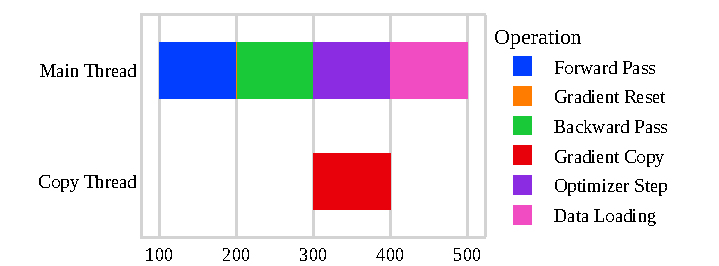
\includegraphics[width=\linewidth]{figures/solution/gradient_copy_timeline_img.pdf}
    \caption{\small{{Schematic representation of asynchronous gradient offloading for efficient sensitivity computation in \sys.}}}
    \label{fig:gradient-copy-timeline} 
\end{figure}





















